\documentclass[a4paper]{report}
\usepackage[dutch]{babel}   % Taal van het document (opmaakregels ed.)
\usepackage{graphicx}
\usepackage{color}

\usepackage{url}                % Opmaak van URLs
%\usepackage[official]{eurosym}  % Euro symbool
%\usepackage{colortbl}           % Kleur tabellen

\usepackage{nonfloat}            % Voeg non-floating tables & figures toe
\usepackage{pdfpages}            % Maak dat voorblad kan toegevoegd worden
\usepackage{amsmath,amsfonts}    % Wiskunde
\usepackage{listings}            % Code Listings

\usepackage{tikz}	% Graphics framework
\usetikzlibrary{positioning}
\usetikzlibrary{calc}

% Substring macro
\def\substring#1#2#3{%
  \expandafter\subm\romannumeral#3000x.{}#1\relax\relax{#2}}
\def\subm#1#2.#3#4\relax#5\relax{%
  \csname sub#1\endcsname#2.#4\relax#5#3\relax}
\def\subx#1.#2\relax#3\relax#4{%
  \expandafter\submb\romannumeral#4000x.{}{}#3\relax}
\def\submb#1#2.#3{\csname sub#1b\endcsname#2.}
\def\subxb#1.#2\relax{#2}

% Karnaugh map macro
% For now, first command (size) is ignored, only 2x2 maps are drawn.
\newcounter{karnaughgrid}
\newcounter{karnaughcount}

\newcounter{karnaughsize}
\newcounter{karnaughsizex}
\newcounter{karnaughsizey}

\newcommand{\kmap}[6]{%
\setcounter{karnaughsize}{#1}

\begin{tikzpicture}
	\setcounter{karnaughgrid}{0};
	\setcounter{karnaughcount}{0};

	\ifcase\value{karnaughsize}
		% Size 0
		\exit
	\or
		% Size 1
		\setcounter{karnaughsizex}{2}
		\setcounter{karnaughsizey}{1}
	\or
		% Size 2
		\setcounter{karnaughsizex}{2};
		\setcounter{karnaughsizey}{2};
	\or
		% Size 3
		\setcounter{karnaughsizex}{4}
		\setcounter{karnaughsizey}{2}
	\else
		\exit	% Wrong size
	\fi

	% Background grid
	\draw	(0,0) grid (\arabic{karnaughsizex},\arabic{karnaughsizey});

	% Set named node at each grid point
	\foreach \y in {\arabic{karnaughsizey},...,0} {
		\foreach \x in {0,...,\arabic{karnaughsizex}} {
			\node (G\arabic{karnaughgrid}) at (\x, \y) {};
			\addtocounter{karnaughgrid}{1};
		}
	}

	% Counting starts at 0, so lower size counters
	\addtocounter{karnaughsizex}{-1};
	\addtocounter{karnaughsizey}{-1};

	\foreach \y in {\arabic{karnaughsizey},...,0} {
		\foreach \x in {0,...,\arabic{karnaughsizex}} {
			\node (I\arabic{karnaughcount}) at (\x, \y) [above right=-1.5pt and -1.5pt] {\tiny \arabic{karnaughcount}};
			\addtocounter{karnaughcount}{1};

			\node at (\x + 0.5, \y + 0.5) {\large $ \substring{#2}{\arabic{karnaughcount}}{\arabic{karnaughcount}} $};
		}
	}

	% Draw variable names
	\ifcase\value{karnaughsize}
		% No zero size maps
	\or
		% Size 1 maps
		\draw[arrows=|-|] ($(node cs:name=G1, anchor=north) + (0, 3pt)$) -- node[above] {$#4$} ($(node cs:name=G2, anchor=north)  + (0, 3pt)$);
	\or
		% Size 2 maps
		\draw[arrows=|-|] ($(node cs:name=G1, anchor=north) + (0, 3pt)$) -- node[above] {$#4$} ($(node cs:name=G2, anchor=north)  + (0, 3pt)$);
		\useasboundingbox; % Set bounding box to current size for nicer centering

		\draw[arrows=|-|] ($(node cs:name=G3, anchor=west) + (-3pt, 0)$) -- node[left] {$#5$} ($(node cs:name=G6, anchor=west)  + (-3pt, 0)$);
	\else
	\draw[arrows=|-|] ($(node cs:name=G1, anchor=north) + (0, 3pt)$) -- node[above] {$#4$} ($(node cs:name=G3, anchor=north)  + (0, 3pt)$);
		\draw[arrows=|-|] ($(node cs:name=G2, anchor=north) + (0, 23pt)$) -- node[above] {$#5$} ($(node cs:name=G4, anchor=north)  + (0, 23pt)$);
		\useasboundingbox; % Set bounding box to current size for nicer centering

		\draw[arrows=|-|] ($(node cs:name=G5, anchor=west) + (-3pt, 0)$) -- node[left] {$#6$} ($(node cs:name=G10, anchor=west)  + (-3pt, 0)$);
	\fi
	
	% Draw extra stuff (like minimizations)
	#3
\end{tikzpicture}}

% Plaats van afbeeldingen
\graphicspath{{images/}}
\DeclareGraphicsExtensions{.pdf,.eps,.png}

% Stel paginastijl in
\pagestyle{headings}

% Zet hier de woorden waarmee de splitser problemen heeft:
\hyphenation{}

% Regel nummering van figuren
\renewcommand{\thefigure}{\thechapter.\arabic{figure}}
\newcommand{\Chapter}[1]{\chapter{#1} \setcounter{figure}{0}}

% Citatie commando voor figuren
\newcommand{\reffig}[1]{Fig.~\ref{#1}}

% Listings setup
\definecolor{darkkeyword}{rgb}{0,0.08,0.40} %Requires the color package.
\definecolor{gray}{gray}{0.7}

\lstdefinelanguage{gezel}{
  tabsize=3,
  frame=single,
  basicstyle=\footnotesize\ttfamily,
  rulecolor=\color{gray},
  identifierstyle=, % nothing happens
  commentstyle=\color{gray}, % red comments
  stringstyle=\color{gray},%\ttfamily, % typewriter type for strings
  showstringspaces={false}, % no special string spaces
  morecomment=[l]{//},
  morestring=[b]",
  morekeywords={always, dp, in, out, tc, ns, reg, sig, sfg, hardwired, sequencer,
                fsm, use, ipblock, ipparm, iptype, lookup, initial, state, system,
                if, then, else, stimulus},
                keywordstyle=\color{blue}\bfseries,classoffset=1,
  morekeywords={\$display, \$cycle, \$dec, \$bin, \$dp, \$finish,
                \$hex, \$sfg, \$trace, \$option},
                keywordstyle=\color{darkkeyword}\bfseries,classoffset=0
}

\lstset{language=gezel,
        showstringspaces=false,
        frameround=ftft,
        captionpos=b,
        xleftmargin=-1cm,
        xrightmargin=-1cm,
        numbers=left,
        numberstyle=\tiny,
        stepnumber=5,
        numberfirstline=true,
        firstnumber=1
}

\renewcommand*\lstlistlistingname{Lijst van listings}

% BibTex opmaak
\bibliographystyle{abbrvurl}

% Voorkom lelijke opmaak
\clubpenalty=8000
\widowpenalty=8000
\displaywidowpenalty=8000

\hyphenpenalty=5000
\tolerance=1000

%%% Code voor figuren %%%
%%% Plaatst figuur op huidige plaats %%%
%
%\vspace{\textfloatsep}
%\begin{minipage}{\linewidth}
%    \begin{center}
%    \includegraphics[width=311px]{fig}
%    \figcaption{Figuur uitleg}\label{Figuur label}
%    \end{center}
%    \end{minipage}
%\vspace{\textfloatsep}

\begin{document}

% Voeg voorblad toe
%
\includepdf{voorblad.pdf}

% Reset counter & maak inhoudstafel
\setcounter{page}{1}
\tableofcontents
\listoffigures
\listoftables
\clearpage

% Include gedeelte (begint op nieuwe pagina
% Indien gewoon invoegen op huidige plaats \input

\Chapter{Inleiding}

 In dit inleidende hoofdstuk zal enige achtergrond informatie verschaft worden omtrent cryptografie. Verder wordt het concept identiteitsgebaseerde cryptografie duidelijk gemaakt. Er zal uitgelegd worden waarom de recente ondekking van pairings hier zo belangrijk voor is. Ten slotte geeft een kort overzicht aan wat in de literatuur terug te vinden is qua implementaties van pairings. In het volgende hoofdstuk wordt de werking van pairings dan wiskundig uitgespit.

\section{Basisachtergrond cryptografie}

Sinds het begin der tijden is er een nood geweest aan manieren om berichten versleuteld te verzenden tussen twee partijen. Voorbeelden van enkele klassieke encryptiemethoden zijn het Atbashcijfer~\cite{athbash} (Babyloni\"e, 600 v.\ Chr.), het Caesarcijfer~\cite{caesar} (Rome, 56 n.\ Chr.) en het dubbele transpositiecijfer~\cite{kahn} (o.a.\ gebruikt door weerstandsgroepen in WO II). E\'en eigenschap die al deze methodes met elkaar gemeen hebben, is het gebruik van dezelfde sleutel voor versleutelen en ontcijferen. Ook vele moderne encryptiemethodes, zoals bijvoorbeeld 3DES~\cite{3des} en AES~\cite{aes}, gebruiken dit principe, dat men symmetrische versleuteling noemt.

In \reffig{fig-encryptie-applicaties-sym-cipher} wordt de algemene werking van een symmetrische encryptie getoond. Alice zendt een bericht M naar Bob door het te versleutelen, vercijferd met een door hen beiden gekende sleutel $k$. Bob op zijn beurt ontcijfert met diezelfde sleutel de cijfertekst C. Indien Eve de vooraf afgesproken sleutel kent, kan zij alle communicatie tussen Alice en Bob ontcijferen. Er is dus nood aan een manier om veilig een sleutel $k$ te kunnen afspreken tussen twee partijen.

\begin{figure}[h]
	\centering
		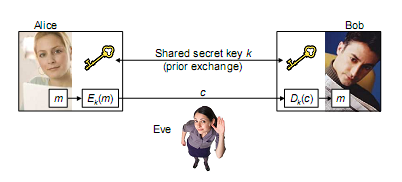
\includegraphics[scale=1.4]{symmetric-cipher-model}
		\caption{Algemene werking van symmetrische encryptie\label{fig-encryptie-applicaties-sym-cipher}}
\end{figure}

Een oplossing voor het veilig afspreken van een gedeelde sleutel was tot 1976 niet gekend. Toen stelden Diffie en Hellman hun algoritme voor sleuteluitwisseling over een onbeveiligd kanaal voor \cite{diffie-hellman}. Deze ontdekking plaveide de weg voor asymmetrische cryptografie (ook wel publieke sleutel cryptografie genoemd). Met behulp van dit type cryptografie kunnen eveneens boodschappen versleuteld worden. Dit wordt ge\"illustreerd in \reffig{fig-encryptie-applicaties-asym-cipher}. Wanneer Alice een bericht M naar Bob wil versturen, zoekt ze eerst zijn publieke sleutel $k_P$ op in een databank. Vervolgens versleutelt ze haar bericht met die publieke sleutel. Enkel Bob kan met behulp van zijn geheime sleutel $k_G$ dan het bericht ontcijferen. Een systeem als dit biedt het grote voordeel dat er geen nood is om de gebruikte (publieke) sleutel geheim te houden. Het is namelijk onmogelijk om met de publieke sleutel de cijfertekst te ontcijferen. Eve heeft er in dit geval dus geen baat bij de gebruikte publieke sleutel te onderscheppen. 

\begin{figure}[h]
	\centering
		 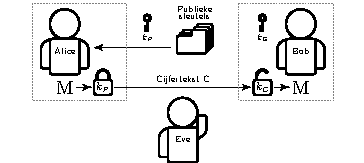
\includegraphics[scale=1.4]{asymmetric-cipher-model}
		 \caption{Algemene werking van asymmetrische encryptie\label{fig-encryptie-applicaties-asym-cipher}}
\end{figure}

Een andere toepassing van asymmetrische cryptografie is het plaatsen en verifi\"eren van digitale handtekeningen. Digitale handtekeningen zijn vergelijkbaar met klassieke handtekeningen. Ze kunnen, indien juist ge\-\"im\-ple\-men\-teerd, gebruikt worden om te verifi\"eren dat een bepaald bericht effectief door de persoon verstuurd is die de verzender beweert te zijn. Ook kan men aan de hand van een digitale handtekening nagaan of de inhoud van een bericht niet gewijzigd werd door een derde persoon tijdens de verzending. ECDSA \cite{ecdsa} en RSA \cite{rsa} zijn enkele van de vele cryptografische algoritmes die toelaten digitale handtekeningen te genereren.

Om te verzekeren dat de publieke sleutels van elke mogelijke ontvanger voorradig zijn, dient een soort een centrale databank voorzien te worden. Indien iemand het voor anderen mogelijk wil maken hem versleutelde berichten te versturen, genereert die persoon eerst een publieke en private sleutel. De publieke sleutel wordt vervolgens naar de database gestuurd, waar iedereen hem kan ophalen.

\section{Identiteitsgebaseerde cryptografie}

Een nadeel van de publieke sleutel cryptografie zoals voorgesteld in de vorige paragraaf zit hem in het sleutelbeheer. Er is geen manier om zeker te zijn dat wanneer de publieke sleutel van Bob opgevraagd wordt de verkregen sleutel effectief die van Bob is. Indien Eve bijvoorbeeld haar publieke sleutel in de database laat opslaan onder Bobs naam, zal Alice berichten voor Bob versleutelen met Eves publieke sleutel. Een mogelijke oplossing hiervoor is bijvoorbeeld het ``web of trust'', zoals ge\"implementeerd door de software PGP \cite{pgp}. Daarbij kunnen mensen aangeven of ze een bepaalde publieke sleutel betrouwbaar vinden of niet. Een sleutel die vergezeld wordt van meerdere getuigenissen van betrouwbaarheid zal dat dan waarschijnlijk ook zijn. Verder bestaat er een zogenaamde ``revocation list'', die aangeeft welke sleutels niet meer geldig zijn.

Uiteraard is ook zo een systeem niet volledig waterdicht. Iemand kan bijvoorbeeld onder verschillende identiteiten sleutels insturen en vervolgens met al die verschillende identiteiten zijn sleutels een certificaat van vertrouwen geven. Indien iemands publieke sleutel zou afgeleid kunnen worden van bekende gegevens omtrent zijn identiteit dan zouden deze problemen niet bestaan.

In 1984 stelde Shamir een methode voor waarbij dit mogelijk zou zijn \cite{shamir}. Het basisidee is als volgt: in plaats van een centrale databank voor publieke sleutels is er een centrale server die private sleutels voor elke gebruiker genereert aan de hand van geheime parameters. Gebruikers kunnen hun private sleutel dus niet zelf berekenen. De centrale server publiceert ook informatie omtrent hoe iemands identiteitsgegevens kunnen worden omgezet naar een publieke sleutel. Wanneer een gebruiker wil deelnemen aan beveiligde communicatie, meldt hij zich aan bij de centrale server en verkrijgt hij zijn private sleutel alsook de parameters om publieke sleutels te berekenen. Voor zowel de private sleutel als de parameters wordt er van uit gegaan dat deze levenslang gelden. Een gebruiker dient zich dus slechts \'e\'enmalig aan te melden.

Uiteraard is ook dit concept niet zonder problemen. Indien bijvoorbeeld de geheime parameters van de centrale server achterhaald worden, is het onmogelijk gebruikers daarvan op de hoogte te brengen. Een mogelijke oplossing is elke gebruiker om de zoveel tijd te voorzien van een nieuwe geheime sleutel. In dat geval stelt zich echter een nieuw probleem, want dan moet een methode bedacht worden om alle nieuwe sleutels bij de gebruikers te krijgen. 

Door deze problemen is de toepassing van identiteitsgebaseerde cryptografie eerder geschikt voor kleine groepen mensen, bijvoorbeeld intern in een bedrijf. In dat geval kost het weinig moeite iedereen op regelmatige tijdstippen van nieuwe sleutels te voorzien.

Een andere ideale toepassing is het gebruik van dit type cryptografie in netwerken van sensoren. Zo'n netwerk kan bestaan uit honderden nodes met een beperkte reken- en vermogenscapaciteit. Indien publieke sleutel cryptografie als vanouds zou worden gebruikt, zou dit leiden tot veel extra communicatie tussen de nodes en een centrale server. Telkens de nodes meetgegevens naar de server willen sturen, zouden ze diezelfde server eerst moeten contacteren om zijn publieke sleutel te weten te komen. In het omgekeerde geval zou de server telkens hij een node wil contacteren hetzelfde moeten doen.  Als echter identiteitsgebaseerde cryptografie wordt toegepast, is al die extra communicatie niet meer nodig, aangezien men de benodigde publieke sleutels kan berekenen met behulp van een unieke ID.

Een uitvoerig overzicht van identiteitsgebaseerde cryptografie en de bijhorende mogelijkheden en problemen valt buiten het bestek van thesis. In het volgende hoofdstuk zullen wel enkele mogelijkheden naderbij bestudeerd worden. Een uitstekend startpunt voor meer informatie is \cite{maas}.

\section{Pairings\label{inleiding-pairings}}

Hoewel het idee reeds in 1984 gepubliceerd werd, zou het echter tot 2001 duren eer Boneh en Franklin een effici\"ent algoritme voor identiteitsgebaseerde cryptografie voorstelden \cite{boneh}. Zij stelden een schema op dat toeliet de idee\"en van Shamir ook effectief te implementeren. In hun voorstel maakten ze gebruik van de Weil pairing \cite{weil}. Al gauw verschenen er variaties op het oorspronkelijke schema. Daarin werd het gebruik van andere pairings voorgesteld, zoals bijvoorbeeld de Tate \cite{tate} of de $\eta_T$ \cite{eta} pairing. Wat pairings juist zijn en hoe ze gebruikt kunnen worden, zal in het volgende hoofdstuk uitvoerig aan bod komen.

Alvorens de wiskunde achter pairings in te duiken, wordt eerst nog een overzicht gegeven van de huidige ``state of the art'' van implementaties van pairings. De mogelijkheden van implementaties op een microchip en een FPGA passeren de revue. Implementaties van pairings op computers zijn per definitie niet in een omgeving met beperkte ressources toepasbaar. Ze hebben dus weinig te maken met deze thesis, die als uitgangspunt compacte implementaties heeft. Vandaar dat dit type implementaties dan ook niet bestudeerd zal worden.

\subsection{Microchip implementaties}

Implementaties van pairings voor gebruik op een MICA node \cite{mica}, specifiek ontwikkeld voor gebruik in netwerken van sensoren, worden voorgesteld in \cite{tinytate}, \cite{tinypbc} en \cite{nanoecc}. De processor op deze node is een ATMega128L microchip \cite{atmega}. Een overzicht van de resultaten is gegeven in \reftbl{tabel-resultaten-sensor}. Rekening houdend met het stroomverbruik en de batterijspanning gegeven in \cite{nanoecc}, is het vermogenverbruik waarschijnlijk ongeveer $23.60$ $mW$.

\begin{table}[h]
	\caption[Resultaten uit de literatuur voor implementaties ontwikkeld op een MICA node]{Resultaten uit de literatuur voor implementaties ontwikkeld op een MICA node \cite{mica}}
	\label{tabel-resultaten-sensor}

	\centering
	\begin{tabular}{lllll}
		\toprule
		& \multirow{2}{*}{TinyTate \cite{tinytate}}	& \multirow{2}{*}{TinyPBC \cite{tinypbc}} &	\multicolumn{2}{c}{NanoECC \cite{nanoecc}}\\
		\cmidrule{4-5}
		& & & \multicolumn{1}{c}{Binair} & \multicolumn{1}{c}{Priem}\\
			\midrule
		Veld					& $\mathbb{F}_{p}$ 256 bit	& $\mathbb{F}_{2^{271}}$	& $\mathbb{F}_{2^{163}}$	& $\mathbb{F}_{p}$ 160 bit\\
		Pairing				& Tate							& $\eta_T$ 						& Tate							& Tate\\
		Rekentijd ($s$)	& 30.21							& 5.45							& 10.96							& 17.93\\
		\bottomrule
	\end{tabular}
\end{table}

\subsection{FPGA implementaties}

In de literatuur zijn vrij veel ontwerpen voor FPGA's terug te vinden. Het probleem is echter dat men zich bij het ontwerp hiervan steeds toelegt op het behalen van een zo hoog mogelijke snelheid, wat resulteert in een grote oppervlakte. Dit type implementaties is dus minder geschikt zijn voor toepassingen met beperkte ressources.

Toch wordt in \reftbl{tabel-resultaten-fpga} een sumier overzicht gegeven van een zeer beperkt aantal ontwerpen. Bij de selectie hiervan werd vooral gekozen voor ontwerpen waarin in een vrij klein veld gerekend werd. Er dient in acht te worden genomen dat bij al deze implementaties snelheid, en niet een compacte, zuinige implementatie, het voornaamste doel is. 

\begin{table}[h]
	\caption{Resultaten uit de literatuur voor implementaties ontwikkeld voor FPGA's}
	\label{tabel-resultaten-fpga}

	\centering
	\begin{tabular}{llllll}
		\toprule
		&	\multicolumn{1}{c}{Veld}	& \multicolumn{1}{c}{Pairing}	& $\begin{array}{@{}c@{}}\text{Opp.}\\\text{[slices]}\end{array}$	& $\begin{array}{@{}c@{}}f\\\text{[MHz]}\end{array}$	& $\begin{array}{@{}c@{}}\text{Reken-}\\\text{tijd }[\mu s]\end{array}$\\
		\midrule
		Ronan \emph{et al.} \cite{ronan}				& $\mathbb{F}_{2^{103}}$	& Tate		& 21021	& 51	& 206\\
		Shu \emph{et al.} \cite{shu}					& $\mathbb{F}_{2^{239}}$	& Tate		& 25287	& 84	& 41\\
		Keller \emph{et al.} \cite{keller}			& $\mathbb{F}_{2^{251}}$	& Tate		& 27725	& 40	& 2370\\
		Grabher en Page \cite{grabher}				& $\mathbb{F}_{3^{97}}$		& Tate		& 4481	& 150	& 432\\
		Beuchat \emph{et al.} \cite{beuchat-eta}	& $\mathbb{F}_{3^{97}}$		& $\eta_T$	& 1833	& 145	& 192\\
		\bottomrule
	\end{tabular}
\end{table}

             % Inleiding
\Chapter{Encryptie - Applicaties}

\emph{Citations needed}

Sinds het begin der tijden is er een nood geweest aan manieren om berichten versleuteld te verzenden tussen twee partijen. Voorbeelden van enkele klassieke encryptiemethoden zijn het Atbashcijfer~\cite{atbash} (Babyloni"e, 600 v. Chr.), het Caesarcijfer~\cite{caesar} (56 n. Chr.) en het dubbele transpositie cijfer~\cite{double-transp} (oa. gebruikt door weerstandsgroepen in WO II). E'en eigenschap die al deze methodes met elkaar gemeen hebben, is het gebruik van een op voorhand afgesproken sleutel. Dit principe, dat ook door vele moderne encryptiemethodes (zoals bv. 3DES~\cite{3DES} en AES~\cite{AES}) gebruikt wordt, noemt men symetrische versleuteling.

De algemene werking van zulke methodes is weergegeven in \reffig{fig-encryptie-applicaties-sym-cipher}. Alice zendt een bericht $m$ naar Bob door het te versleutelen, met een door hen beiden gekende sleutel $k$, die op zijn beurt met diezelfde sleutel het bericht ontcijfert. Indien Eve de vooraf afgesproken sleutel kent, kan zij uiteraard alle communicatie tussen Alice en Bob ontcijferen. Er is dus nood aan een manier om veilig een sleutel $k$ te kunnen afspreken tussen twee partijen. Deze sleutel kan dan vervolgens bijvoorbeeld gebruikt worden in een symmetrisch sleutel algoritme.

\vspace{\textfloatsep}
\begin{minipage}{\linewidth}
    \begin{center}
    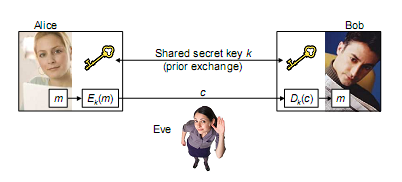
\includegraphics[width=7cm]{symmetric-cipher-model}
    \figcaption{Algemene structuur van een symmetrische versleutelingsmethode}\label{fig-encryptie-applicaties-sym-cipher}
    \end{center}
    \end{minipage}
\vspace{\textfloatsep}

Een oplossing voor dit probleem was niet gekend tot en met 1976, toen Diffie en Hellman hun algoritme voor sleutel uitwisseling~\cite{diffie-hellman} publiceerden. Hun algoritme laat twee partijen toe een geheime sleutel over een onbeveiligd kanaal af te spreken. Deze ontdekking plaveide de weg voor talrijke publieke sleutel methodes (oftewel asymmetrische sleutel methodes), waarvan de werking wordt getoond in \reffig{fig-encryptie-applicaties-asym-cipher}.

\vspace{\textfloatsep}
\begin{minipage}{\linewidth}
    \begin{center}
    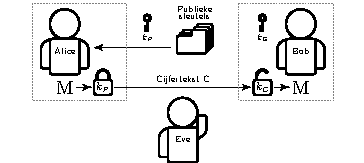
\includegraphics[width=7cm]{asymmetric-cipher-model}
    \figcaption{Algemene structuur van een asymmetrische versleutelingsmethode}\label{fig-encryptie-applicaties-asym-cipher}
    \end{center}
    \end{minipage}
\vspace{\textfloatsep} % Encryptie - Applicaties van encryptie
\Chapter{Encryptie - Wiskundige Achtergrond}

Lees alles maar in \cite{maas}.    % Encryptie - Wiskundige achtergrond
\Chapter{Modular Arithmetic Logic Unit (MALU)}

\section{MALU over GF($2^m$)}

\vspace{\textfloatsep}
\begin{minipage}{\linewidth}
    \begin{center}
    \beginpgfgraphicnamed{malu-core-basic}
      \begin{tikzpicture}
\tikzset {
	xor/.style={draw, xor gate US, logic gate inputs=nn, rotate=90, xscale=-1, line width=0.6pt},
	labelbox/.style={draw, chamfered rectangle, chamfered rectangle corners={north east, south east}, chamfered rectangle angle=55, chamfered rectangle xsep=2cm, chamfered rectangle ysep=14pt/2, minimum height=14pt, minimum width=1.2cm, text width=1cm, inner sep=0pt, text ragged},
	labelboxin/.style={labelbox, anchor=base},
	labelboxout/.style={labelbox, anchor=west},
	joint/.style={inner sep=0mm, outer sep=0pt, text height=0mm, text width=0mm, minimum height=0.15cm, fill, circle},
	dots/.style={},
	bit/.style={line width=0.8pt, line cap=rect},
	multibit/.style={line width=2pt},
	nothing/.style={inner sep=0mm, outer sep=0pt, text width=0mm, text height=0mm, minimum width=0.8pt},
	labeltext/.style={text ragged},
	labeltextin/.style={labeltext, anchor=west, xshift=-6mm},
	labeltextout/.style={labeltext, anchor=west, xshift=0mm}
}

\matrix [column sep=1.5mm, row sep=1.5mm] {
	\node[labeltextin] {T$_i$}; \node[labelboxin] (i1) {}; &
	&[1mm]
	\node[joint, xshift=-0.18cm/2] (j1) {}; &
	\node[joint, xshift=-0.18cm/2] (j2) {}; &
	\node[joint, xshift=-0.18cm/2] (j3) {}; &
	\node[joint, xshift=-0.18cm/2] (j4) {}; &
	\node[dots] (e1) {$\ldots$}; &
	\node[nothing, xshift=-0.18cm/2] (j5) {}; \\

	\node[labeltextin] {A$_i$B}; \node[labelboxin] (i2) {}; &
	&
	\node[joint, xshift=0.18cm/2] (j6) {}; &
	\node[joint, xshift=0.18cm/2] (j7) {}; &
	\node[joint, xshift=0.18cm/2] (j8) {}; &
	\node[joint, xshift=0.18cm/2] (j9) {}; &
	\node[dots] (e2) {$\ldots$}; &
	\node[nothing, xshift=0.18cm/2] (j10) {}; \\[-1mm]

	&
	&
	\node[xor] (x1) {}; &
	\node[xor] (x2) {}; &
	\node[xor] (x3) {}; &
	\node[xor] (x4) {}; &
	\node (e3) {}; &
	\node[xor] (x5) {}; \\[-1mm]

	\node[labeltextin] {m$_i$P}; \node[labelboxin] (i3) {}; &
	&
	\node[joint, xshift=0.18cm] (j11) {}; &
	\node[joint, xshift=0.18cm] (j12) {}; &
	\node[joint, xshift=0.18cm] (j13) {}; &
	\node[joint, xshift=0.18cm] (j14) {}; &
	\node[dots] (e4) {$\ldots$}; &
	\node[nothing, xshift=0.18cm] (j15) {}; \\[-1mm]

	&
	&
	\node[xor, yshift=-0.18cm/2] (x6) {}; &
	\node[xor, yshift=-0.18cm/2] (x7) {}; &
	\node[xor, yshift=-0.18cm/2] (x8) {}; &
	\node[xor, yshift=-0.18cm/2] (x9) {}; &
	\node (e5) {}; &
	\node[xor, yshift=-0.18cm/2] (x10) {}; \\[-2mm]

	\node[nothing, xshift=4mm] (i4) {}; &
	\node[nothing, xshift=4mm] (e6) {}; &
	\node[nothing, xshift=4mm] (e7) {}; &
	\node[nothing, xshift=4mm] (e8) {}; &
	\node[nothing, xshift=4mm] (e9) {}; &
	\node[nothing, xshift=4mm] (e10) {}; &
	\node[dots] (e11) {$\ldots$}; &
	&[4mm]
	\node[labeltextout] {m$_{i+1}$}; \node[labelboxout] (o1) {}; \\

	&
	\node[nothing, xshift=0.5cm] (j16)	{}; &
	\node[joint, xshift=0.8cm] (j17) {}; &
	\node[joint, xshift=0.8cm] (j18) {}; &
	\node[joint, xshift=0.8cm] (j19) {}; &
	\node[joint, xshift=0.8cm] (j20) {}; &
	\node[dots] (e12) {$\ldots$}; &
	\node[joint, xshift=-0.5cm] (j21) {}; &
	\node[labeltextout] {T$_{i+1}$}; \node[labelboxout] (o2) {}; \\
};

\path[-] (i1.east) edge [multibit, line cap=rect] (j1.base)
			(j1.base) edge [multibit] (j2.base)
			(j2.base) edge [multibit] (j3.base)
			(j3.base) edge [multibit] (j4.base)
			(j4.base) edge [multibit] (e1)
			(e1) edge [multibit] (j5.east)

			(i2.east) edge [multibit, line cap=rect] (j6.base)
			(j6.base) edge [multibit] (j7.base)
			(j7.base) edge [multibit] (j8.base)
			(j8.base) edge [multibit] (j9.base)
			(j9.base) edge [multibit] (e2)
			(e2) edge [multibit] (j10.east)

			(j1.base) edge [bit] (x1.input 1)
			(j6.base) edge [bit] (x1.input 2)

			(j2.base) edge [bit] (x2.input 1)
			(j7.base) edge [bit] (x2.input 2)

			(j3.base) edge [bit] (x3.input 1)
			(j8.base) edge [bit] (x3.input 2)

			(j4.base) edge [bit] (x4.input 1)
			(j9.base) edge [bit] (x4.input 2)

			(j5.base) edge [bit] (x5.input 1)
			(j10.base) edge [bit] (x5.input 2)

			(i3.east) edge [multibit, line cap=rect] (j11.base)
			(j11.base) edge [multibit] (j12.base)
			(j12.base) edge [multibit] (j13.base)
			(j13.base) edge [multibit] (j14.base)
			(j14.base) edge [multibit] (e4)
			(e4) edge [multibit] (j15.east)

			(x1.output) edge [bit] (x6.input 1)
			(j11.base) edge [bit] (x6.input 2)

			(x2.output) edge [bit] (x7.input 1)
			(j12.base) edge [bit] (x7.input 2)

			(x3.output) edge [bit] (x8.input 1)
			(j13.base) edge [bit] (x8.input 2)

			(x4.output) edge [bit] (x9.input 1)
			(j14.base) edge [bit] (x9.input 2)

			(x5.output) edge [bit] (x10.input 1)
			(j15.base) edge [bit] (x10.input 2)

			(j16.west) edge [multibit] (j17.base)
			(j17.base) edge [multibit] (j18.base)
			(j18.base) edge [multibit] (j19.base)
			(j19.base) edge [multibit] (j20.base)
			(j20.base) edge [multibit] (e12)
			(e12) edge [multibit] (j21.base)
			(j21.base) edge [multibit] (o2.west);

\draw		[bit] (i4.south east) node [above] {\large $0$} -| (j16.base)
			
			\foreach \i / \j / \k in {6/7/17, 7/8/18, 8/9/19, 9/10/20} {
				(x\i.output) |- (e\j.base) -| (j\k)
			}

			(e11) -| (j21)
			(x10.output) |- (o1.west);

% Draw rectangle
\draw[multibit, color=black!50] ($(j1.north west) + (-7mm, 3mm)$) rectangle ($(o2.south west) + (-3mm, 0)$);
\end{tikzpicture}

    \endpgfgraphicnamed
    \figcaption{Basis implementatie van een MALU-blok met $d = 1$}
    \label{fig-malu-core-basic}
    \end{center}
    \end{minipage}
\vspace{\textfloatsep}

\vspace{\textfloatsep}
\begin{minipage}{\linewidth}
    \begin{center}
    \beginpgfgraphicnamed{malu-core-optimized}
      \tikzset {
	xor/.style={draw, xor gate US, logic gate inputs=nn, rotate=90, xscale=-1, line width=0.6pt},
	labelbox/.style={draw, chamfered rectangle, chamfered rectangle corners={north east, south east}, chamfered rectangle angle=55, chamfered rectangle xsep=2cm, chamfered rectangle ysep=14pt/2, minimum height=14pt, minimum width=1.2cm, text width=1cm, inner sep=0pt, text ragged},
	labelboxin/.style={labelbox, anchor=base},
	labelboxout/.style={labelbox, anchor=west},
	joint/.style={inner sep=0mm, outer sep=0pt, text height=0mm, text width=0mm, minimum height=0.15cm, fill, circle},
	dots/.style={},
	bit/.style={line width=0.8pt, line cap=rect},
	multibit/.style={line width=2pt},
	nothing/.style={inner sep=0mm, outer sep=0pt, text width=0mm, text height=0mm, minimum width=0.8pt},
	labeltext/.style={text ragged},
	labeltextin/.style={labeltext, anchor=west, xshift=-6mm},
	labeltextout/.style={labeltext, anchor=west, xshift=0mm}
}

\begin{tikzpicture}
\matrix [column sep=1.5mm, row sep=1.5mm] {
	\node[labeltextin] {T$_i$}; \node[labelboxin] (i1) {}; &
	&[1mm]
	\node[joint, xshift=-0.18cm/2] (j1) {}; &
	\node[joint, xshift=-0.18cm/2] (j2) {}; &
	\node[joint, xshift=-0.18cm/2] (j3) {}; &
	\node[joint, xshift=-0.18cm/2] (j4) {}; &
	\node[dots] (e1) {$\ldots$}; &
	\node[nothing, xshift=-0.18cm/2] (j5) {}; \\

	\node[labeltextin] {A$_i$B}; \node[labelboxin] (i2) {}; &
	&
	\node[joint, xshift=0.18cm/2] (j6) {}; &
	\node[joint, xshift=0.18cm/2] (j7) {}; &
	\node[joint, xshift=0.18cm/2] (j8) {}; &
	\node[joint, xshift=0.18cm/2] (j9) {}; &
	\node[dots] (e2) {$\ldots$}; &
	\node[nothing, xshift=0.18cm/2] (j10) {}; \\[-1mm]

	&
	&
	\node[xor] (x1) {}; &
	\node[xor] (x2) {}; &
	\node[xor] (x3) {}; &
	\node[xor] (x4) {}; &
	\node (e3) {}; &
	\node[xor] (x5) {}; \\[-1mm]

	\node[labeltextin] {m$_i$}; \node[labelboxin] (i3) {}; &
	&
	\node[joint, xshift=0.18cm] (j11) {}; &
	&
	&
	\node[joint, xshift=0.18cm] (j14) {}; &
	\node[dots] (e4) {$\ldots$}; &
	\node[nothing, xshift=0.18cm] (j15) {}; \\[-1mm]

	&
	&
	\node[xor, yshift=-0.18cm/2] (x6) {}; &
	&
	&
	\node[xor, yshift=-0.18cm/2] (x9) {}; &
	\node (e5) {}; &
	\node[xor, yshift=-0.18cm/2] (x10) {}; \\[-2mm]

	\node[nothing, xshift=4mm] (i4) {}; &
	\node[nothing, xshift=4mm] (e6) {}; &
	\node[nothing, xshift=4mm] (e7) {}; &
	\node[nothing, xshift=4mm] (e8) {}; &
	\node[nothing, xshift=4mm] (e9) {}; &
	\node[nothing, xshift=4mm] (e10) {}; &
	\node[dots] (e11) {$\ldots$}; &
	&[4mm]
	\node[labeltextout] {m$_{i+1}$}; \node[labelboxout] (o1) {}; \\

	&
	\node[nothing, xshift=0.5cm] (j16)	{}; &
	\node[joint, xshift=0.8cm] (j17) {}; &
	\node[joint, xshift=0.8cm] (j18) {}; &
	\node[joint, xshift=0.8cm] (j19) {}; &
	\node[joint, xshift=0.8cm] (j20) {}; &
	\node[dots] (e12) {$\ldots$}; &
	\node[joint, xshift=-0.5cm] (j21) {}; &
	\node[labeltextout] {T$_{i+1}$}; \node[labelboxout] (o2) {}; \\
};

\path[-] (i1.east) edge [multibit, line cap=rect] (j1.base)
			(j1.base) edge [multibit] (j2.base)
			(j2.base) edge [multibit] (j3.base)
			(j3.base) edge [multibit] (j4.base)
			(j4.base) edge [multibit] (e1)
			(e1) edge [multibit] (j5.east)

			(i2.east) edge [multibit, line cap=rect] (j6.base)
			(j6.base) edge [multibit] (j7.base)
			(j7.base) edge [multibit] (j8.base)
			(j8.base) edge [multibit] (j9.base)
			(j9.base) edge [multibit] (e2)
			(e2) edge [multibit] (j10.east)

			(j1.base) edge [bit] (x1.input 1)
			(j6.base) edge [bit] (x1.input 2)

			(j2.base) edge [bit] (x2.input 1)
			(j7.base) edge [bit] (x2.input 2)

			(j3.base) edge [bit] (x3.input 1)
			(j8.base) edge [bit] (x3.input 2)

			(j4.base) edge [bit] (x4.input 1)
			(j9.base) edge [bit] (x4.input 2)

			(j5.base) edge [bit] (x5.input 1)
			(j10.base) edge [bit] (x5.input 2)

			(i3.east) edge [bit, line cap=rect] (j11.base)
			(j11.base) edge [bit] (j14.base)
			(j14.base) edge [bit] (e4)
			(e4) edge [bit] (j15.base)

			(x1.output) edge [bit] (x6.input 1)
			(j11.base) edge [bit] (x6.input 2)

			(x4.output) edge [bit] (x9.input 1)
			(j14.base) edge [bit] (x9.input 2)

			(x5.output) edge [bit] (x10.input 1)
			(j15.base) edge [bit] (x10.input 2)

			(j16.west) edge [multibit] (j17.base)
			(j17.base) edge [multibit] (j18.base)
			(j18.base) edge [multibit] (j19.base)
			(j19.base) edge [multibit] (j20.base)
			(j20.base) edge [multibit] (e12)
			(e12) edge [multibit] (j21.base)
			(j21.base) edge [multibit] (o2.west);

\draw		[bit] (i4.south east) node [above] {\large $0$} -| (j16.base)
			
			\foreach \i / \j / \k in {6/7/17, 2/8/18, 3/9/19, 9/10/20} {
				(x\i.output) |- (e\j.base) -| (j\k)
			}

			(e11) -| (j21)
			(x10.output) |- (o1.west);

% Draw rectangle
\draw[multibit, color=black!50] ($(j1.north west) + (-7mm, 3mm)$) rectangle ($(o2.south west) + (-3mm, 0)$);
\end{tikzpicture}

    \endpgfgraphicnamed
    \figcaption{Geoptimaliseerde implementatie van een MALU-blok met $d = 1$}
    \label{fig-malu-core-basic}
    \end{center}
    \end{minipage}
\vspace{\textfloatsep}

\vspace{\textfloatsep}
\begin{minipage}{\linewidth}
    \begin{center}
    \beginpgfgraphicnamed{malu-wrapper-gf2m}
      \tikzset {
	and/.style={draw, and gate US, logic gate inputs=nn, thick, scale=0.8},
	labelbox/.style={draw, chamfered rectangle, chamfered rectangle corners={north east, south east}, chamfered rectangle angle=55, chamfered rectangle xsep=2cm, chamfered rectangle ysep=14pt/2, minimum height=14pt, minimum width=1.2cm, text width=1cm, inner sep=0pt, outer sep=0pt, text ragged},
	labelboxin/.style={labelbox, anchor=base},
	labelboxout/.style={labelbox, anchor=west},
	labelboxreg/.style={draw, minimum height=14pt, minimum width=2cm, outer sep=0pt},
	joint/.style={inner sep=0mm, outer sep=0pt, text height=0mm, text width=0mm, minimum height=0.15cm, fill, circle},
	bit/.style={thick, line cap=butt},
	multibit/.style={line width=2pt},
	nothing/.style={inner sep=0mm, outer sep=0pt, text width=0mm, text height=0mm, minimum width=0.8pt},
	labeltext/.style={text ragged},
	labeltextin/.style={labeltext, anchor=west, xshift=-6mm},
	labeltextout/.style={labeltext, anchor=west, xshift=0mm},
	labeltextreg/.style={labeltext, text centered},
	mux/.style={draw, trapezium, trapezium stretches=true, rotate=-90, inner sep=1pt, minimum height=12pt, minimum width=1.2cm, xshift=2.2mm, outer sep=0pt},
	adder/.style={draw, circle, inner sep=0pt, outer sep=0pt, minimum size=5mm, semithick},
	malucore/.style={draw, minimum height=1.4cm, minimum width=3cm, text width=2cm, text centered, semithick}
}

\def\labelboxregl#1#2#3{\node[labeltextreg, #3] {#2}; \node[labelboxreg, #3] (#1) {}; \draw (#1.north west) -- ($(#1.north west)!0.5!(#1.south west) + (2mm, 0)$) -- (#1.south west);}

\def\labelboxregr#1#2#3{\node[labeltextreg, #3] {#2}; \node[labelboxreg, #3] (#1) {}; \draw (#1.north east) -- ($(#1.north east)!0.5!(#1.south east) + (-2mm, 0)$) -- (#1.south east);}

\def\labelboxin#1#2#3{\node[labeltextin, #3] {#2}; \node[labelboxin, #3] (#1) {};}
\def\labelboxout#1#2#3{\node[labeltextout, #3] {#2}; \node[labelboxout, #3] (#1) {};}

\def\adder#1{\node[adder] (#1) {}; \draw [semithick] (#1.north) -- (#1.south) (#1.west) -- (#1.east);} 

\def\boxmalucore#1{\node[malucore] (#1) {\Large MALU Core};}

\begin{tikzpicture}
\matrix [column sep=1.5mm, row sep=1.5mm] {
	\labelboxin{i1}{start}{}; &[6mm]
	&[6mm]
	\labelboxregl{r1}{start}{}; &[-5mm]
	\labelboxregl{r2}{ready}{}; &[8mm] \\

	\labelboxin{i2}{mode}{}; &
	&
	\labelboxregl{r3}{mode}{}; \\

	\labelboxin{i3}{A}{}; &
	\node[joint, xshift=-3mm] (j1) {}; &
	&
	\node[mux, rotate=-90, yshift=2mm](m2){}; 
	\node[joint, xshift=3.1mm] (j3) {};\\

	&
	\node[mux, rotate=-90, yshift=-2.5mm](m1){}; &
	\labelboxregr{r4}{T}{}; &
	\node[joint] (j2) {}; &
	\labelboxout{o1}{out}{};\\

	\labelboxin{i4}{B}{yshift=-1mm}; &
	\node[and, yshift=0mm, xshift=6mm] (a1) {};&
	\boxmalucore{mcore}; 
	\node[joint, xshift=19.1mm, yshift=3mm] (j5) {};
	\node[joint, xshift=19.1mm, yshift=-3mm] (j4) {}; &
	&
	\labelboxout{o2}{ready}{}; \\
	
	&
	&
	\labelboxregr{r5}{m}{}; \\
};

\path[-]	(i1.east) edge [bit, line cap=rect] ($(i1.east)!0.5!(r1.west)$)
			($(i1.east)!0.5!(r1.west)$) edge [bit, line cap=butt] (r1.west)
			(i2.east) edge [bit, line cap=rect] ($(i2.east)!0.5!(r3.west)$)
			($(i2.east)!0.5!(r3.west)$) edge [bit, line cap=butt] (r3.west)
			(i3.east) edge [multibit, line cap=rect] (j1.base)
			(j1.base) edge [bit] ($(m1.south east) + (-1mm, 0)$)
			(i4.east) edge [multibit, line cap=rect] ($(i4.east)!0.5!($(a1.south west) + (0, 1.5mm)$)$)
			($(i4.east)!0.5!($(a1.south west) + (0, 1.5mm)$)$) edge [multibit, line cap=butt] ($(a1.south west) + (0, 1.5mm)$)
			(a1.east) edge [multibit] (mcore.west)
			(r4.east) edge [multibit] (j2.base)
			(j2.base) edge [multibit] (o1.west)
			(j2.base) edge [multibit] (m2.north)
			($(m2.south west) + (1mm, 2mm)$) edge [multibit] ($(m2.south west) + (1mm, 0)$);

\draw		[multibit] (j1.base) -| ($(m2.south east) + (-1mm, 0)$)
			(r4.west) -| ($(mcore.north west) + (-4mm, 0)$) |- ($(mcore.north west) + (0, -4mm)$)
			($(mcore.north east) + (0, -4mm)$) -| ($(m2.south west) + (6mm, 0)$) |- ($(m2.south) + (0, 2mm)$) -| (m2.south);

\draw		[bit] (m1.north) |- ($(a1.north west) + (0, -1.5mm)$)
			($(mcore.south east) + (4mm, 4mm)$) |- ($(mcore.north east) + (4mm, -4mm)$)
			(m1.south) -- node[at end, above] {0} ($(m1.south) + (0, 3mm)$)
			($(m1.south west) + (1mm, 0)$)-- node[at end, above] {1} ($(m1.south west) + (1mm, 3mm)$);

\draw		[bit] (r5.east) -| ($(mcore.south east) + (4mm, 0)$) |- ($(mcore.south east) + (0, 4mm)$) 
			(r5.west) -| ($(mcore.south west) + (-4mm, 0)$) |- ($(mcore.south west) + (0, 4mm)$)
			(o2.west) -- ($(o2.west) + (-6mm, 0)$);

\draw[multibit, color=black!50] ($(i1.east) + (4mm, 14pt)$) rectangle ($(r5.south east) + (30mm, -6pt)$);
\end{tikzpicture}
    \endpgfgraphicnamed
    \figcaption{GF($2^m$) Wrapper}
    \label{fig-malu-wrapper-gf2m}
    \end{center}
    \end{minipage}
\vspace{\textfloatsep}
                  % Modular Aritmitic Logical Unit - Design
\Chapter{MALU - Uitbreiding Naar Pairings}

         % MALU - Uitbreiding naar pairings
\Chapter{MALU - Pairings - Implementatie}
      % MALU - Pairings hardware implementatie
\Chapter{Optimalisaties}
\subsection{Clock gating voor het A register}

Daar voor het A register gekozen moet worden uit drie  inputs, zijnde A, A$_{\text{in}}$ of A$_{\ll 1}$, is voor dit register een andere implementatie vereist dan voor de overige registers. Daar moet immers slechts uit X of X$_{\text{in}}$ gekozen worden, wat, zoals eerder aangetoond, toelaat een MUX uit te sparen door toepassing van clock gating. In tegenstelling tot de andere registers kan men hier niet anders dan een MUX gebruiken. Ook aan het circuit voor de clock gating moeten enkele toevoegingen gebeuren.

Ten eerste wordt gekeken wat juist de nodige aanpassingen aan het clock gating enable signaal zijn. Indien er vermenigvuldigd wordt (mode $= 0$), moet elke clock cycle A$_{\ll 1}$ in A opgeslagen worden. Het kloksignaal dient dus doorgelaten te worden indien een berekening begint (start $= 1$) of indien een vermenigvuldiging aan de gang is. Dit leidt tot onderstaande Karnaugh map:

%\begin{tabular}{r|c|c|}
%	& \multicolumn{2}{|l}{$mode$} \\
%	$start$ & 0 & 1 \\ \hline
%	0 & 1 & 0 \\ \hline
%	1 & 1 & 1 \\ \hline
%\end{tabular}

\vspace{\textfloatsep}
\begin{minipage}{\linewidth}
	\begin{center}
		\kmap{2}{Clk$_{\text{En}}:$}{{start}{mode}}{1101}{%
			\draw[red] (node cs:name=G0, anchor=south east) rectangle ($(node cs:name=G5, anchor=north west) + (0, 4pt)$);
			\draw[red] ($(node cs:name=G1, anchor=south east) + (3pt, -2pt)$) rectangle ($(node cs:name=G8, anchor=north west) + (-2pt, 3pt)$);%
		}
	\end{center}
\end{minipage}
\vspace{\textfloatsep}

M.a.w.\ het nodige klok enable signaal voor de flip flops is:

\[ \text{Clk}_{\text{En}} = \text{start} + \overline{\text{mode}} \]

Ten tweede wordt gezocht welk signaal gebruikt moet worden om de MUX te schakelen. Bij het starten van een berekening, moet uiteraard A$_{\text{in}}$ geselecteerd worden. Bij de uitvoering van een vermenigvuldiging (mode $= 0$) dient A$_{\ll 1}$ geselecteerd te worden. Wanneer een berekening aan de gang is, maakt het voor een optelling (mode $= 1$) niet uit welke ingang gekozen wordt, aangezien de klok ingang van de flip flop dan uitgeschakeld is. Dit geeft aanleiding tot de volgende Karnaugh map:

\vspace{\textfloatsep}
\begin{minipage}{\linewidth}
	\begin{center}
	\kmap{2}{A$_{\text{sel}}:$}{{start}{mode}}{{A$_{\ll 1}$}{A$_{\text{in}}$}{$-$}{A$_{\text{in}}$}}{%
			\draw[red] ($(node cs:name=G1, anchor=south east) + (2pt, 0)$) rectangle ($(node cs:name=G8, anchor=north west) + (-2pt, 3pt)$);
}
	\end{center}
	\end{minipage}
\vspace{\textfloatsep}

Waarbij het $-$ symbool staat voor een zogenaamde ``don't care''. Indien men A$_{\ll 1}$ aansluit op de 0-ingang van de MUX en A$_{\text{in}}$ op de 1-ingang, kan start dus gebruikt worden als schakelsignaal:

\[ \text{A}_{\text{sel}} = \text{start} \]

         % MALU - Optimalisatie (& parallellisatie)
\Chapter{Tests}
                 % MALU - Oppervlakte/snelheids tests
\Chapter{Veiligheid - Side Channel Attacks}
  % Side channel attack weerstand
\Chapter{Conclusie \& toekomstig onderzoek}

\section{Conclusie}

Deze thesis handelde over pairings, een recente ontwikkeling op gebied van cryptografie die identiteits-gebaseerde cryptografie toelaat. Er werd onderzocht hoe de Tate pairing ge\"implementeerd kan worden in hardware. Meer specifiek werd de nadruk gelegd op een compacte implementatie die daarbovenop nog eens zo weinig mogelijk vermogen verbruikte. Een implementatie van dat type zou toegepast kunnen worden in netwerken van sensoren of toestellen met een beperkt vermogen.

Verscheidene bestaande algoritmen werden aangepast en geoptimaliseerd zodat ze met een minimum gebruik aan geheugen uitgevoerd konden worden. Er werd een geheugenontwerp voorgesteld dat een goed compromis gaf tussen grootte en verbruik. Tevens werden verschillende oppervlakte- en vermogensbesparende technieken toegepast om het uiteindelijke circuit zo goed mogelijk aan de doelstellingen te laten voldoen. Door aanpassing van de kloksnelheid en het aantal gebruikte rekenschakelingen (MALUs) kunnen de parameters van het ontwerp aangepast worden aan de individuele normen van een toepassing.

Het resulterende ontwerp is uniek in zijn soort. Het verbruik per oppervlakte (genormaliseerd voor de werkfrequentie) van het gepresenteerde ontwerp is zeer laag. Ten tijde van dit schrijven waren nog geen andere ontwerpen gepubliceerd waarbij de nadruk op compactheid en laag vermogenverbruik lag.

\section{Toekomstig onderzoek}

Als toekomstig onderzoek kan het interessant zijn te onderzoeken of het mogelijk is het ontwerp nog verder te optimaliseren. Daarbij is het waarschijnlijk nuttig te trachten de gebruikte FSM verder te vereenvoudingen, aangezien die zowat de helft van de oppervlakte van de totale implementatie inneemt.

Verder zou ook onderzocht moeten worden in welke mate het werken over een groter Galois veld de oppervlakte en het verbruik wijzigt. Ook de implementatie van andere types pairings kan interessant zijn. Zo bestaan er bijvoorbeeld de $\eta_T$ en de modified Tate pairing die beiden berekend kunnen worden in ongeveer de helft van de tijd nodig voor de berekening van de Tate pairing.
             % Conclusie

\appendix                       % Start appendices

\Chapter{GEZEL Code}                  % Implementatie code

% BibTex referenties
\bibliography{references}

% Lege achterpagina
\clearpage
\mbox{~}
\thispagestyle{empty}

\end{document}
